\section{Results}

\begin{frame}
    \begin{center}
        \textbf{Application: Reduced-Order Modeling for Ablating Non-Decomposing Thermal Protection Systems}
    \end{center}
\end{frame}

%%%%%%%%%%%%%%%%%%%%%%%%%%%%%%%%% TPS %%%%%%%%%%%%%%%%%%%%%%%%%%%%%%%%%
\begin{frame}{Hypersonic Thermal Protection Systems}
    \footnotesize
    Multi-layered TPS shields structures from extreme aerothermal heating,
    \vspace{-0.1in}
    \begin{figure}
        \centering
        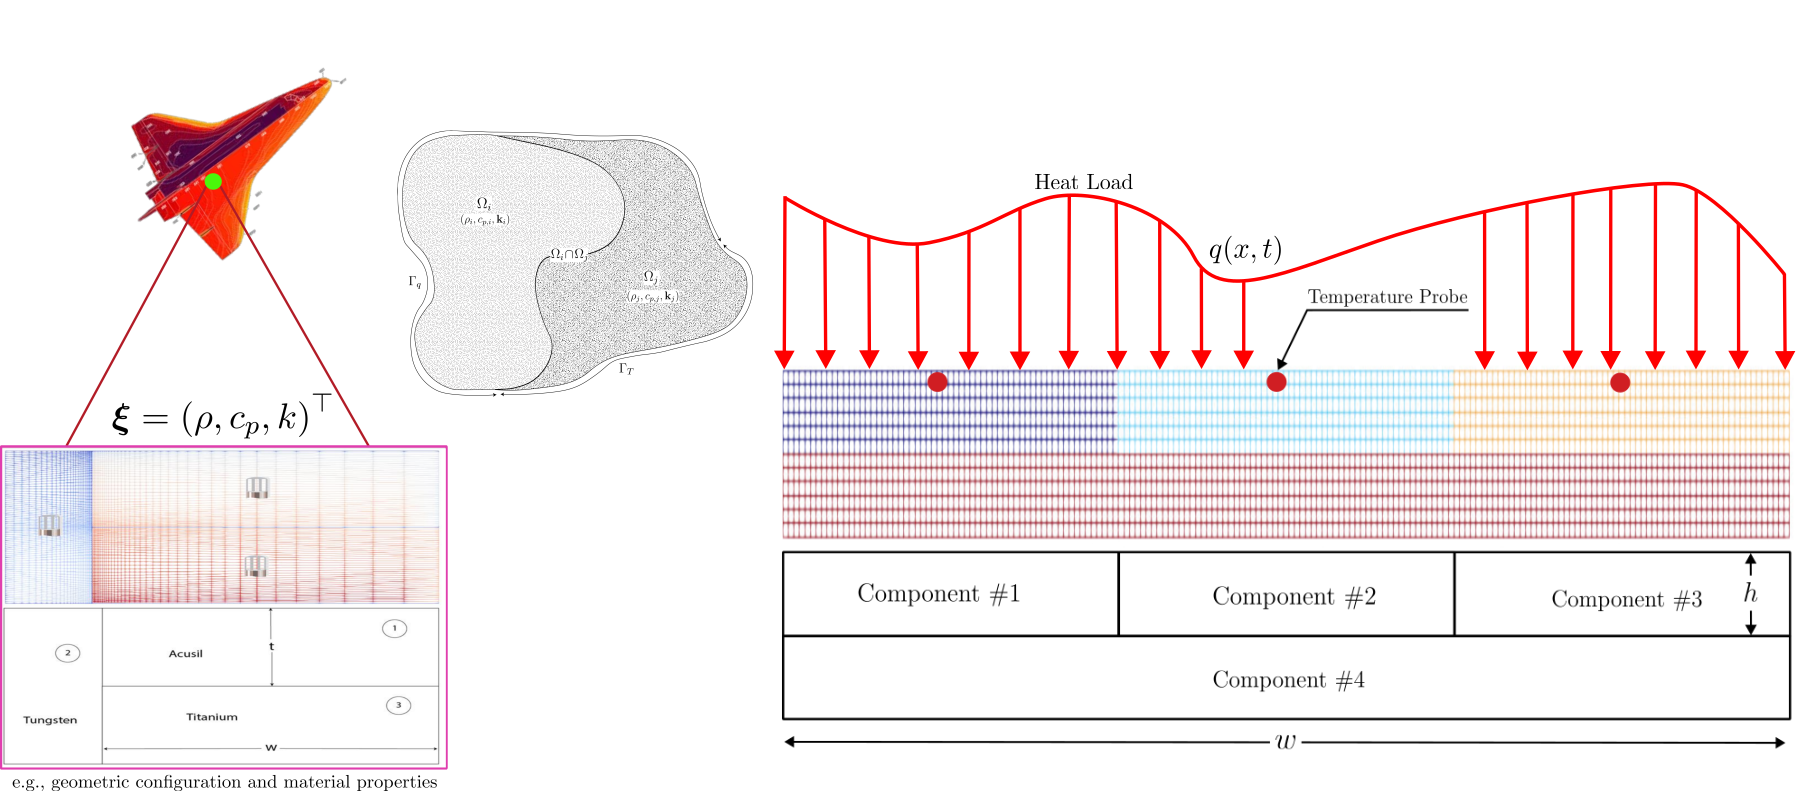
\includegraphics[width=0.9\textwidth]{../figs/ablation/tps.png}
    \end{figure}
\end{frame}

\begin{frame}{Hypersonic Thermal Protection System}
    \footnotesize
    \visible<1->{
    \emph{Full-order model} (FOM) of ablating non-decomposing TPS via FEM,}
    \begin{columns}
        \begin{column}{0.5\textwidth}
            \visible<2->{
            \begin{figure}
                \centering
                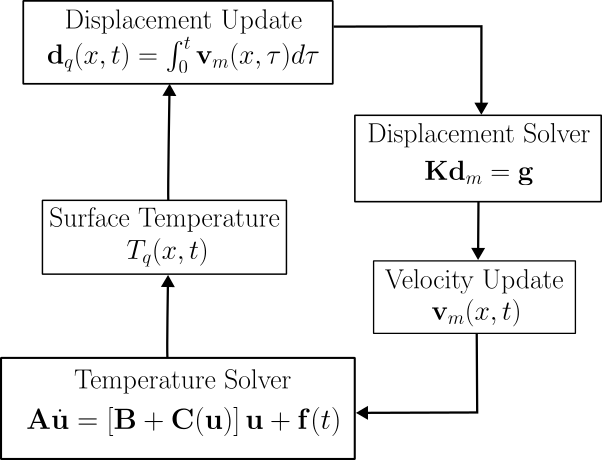
\includegraphics[width=0.9\textwidth]{../figs/ablation/coupling.png}
            \end{figure}
            $\vu$: temperature field, $\vd_m$: mesh displacement field.}
        \end{column}
        \begin{column}{0.4\textwidth}
            \visible<3->{
            Time: $t_0$,
            \begin{figure}
                \centering
                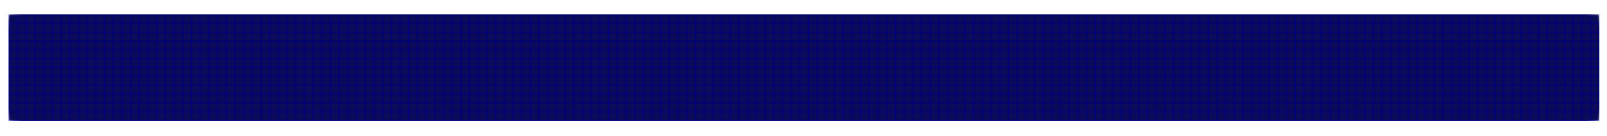
\includegraphics[width=0.9\textwidth]{../figs/ablation/start_time.png}
            \end{figure}}
            \visible<4->{
            Time: $t_f / 2$,
            \begin{figure}
                \centering
                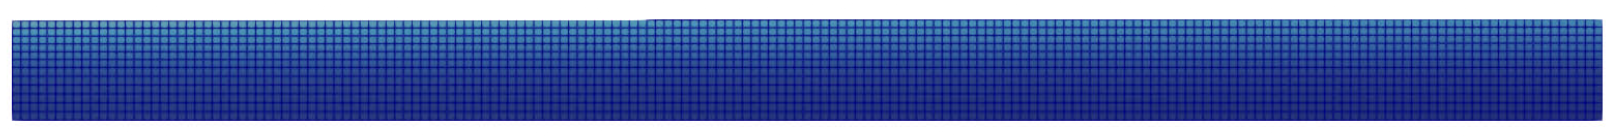
\includegraphics[width=0.9\textwidth]{../figs/ablation/middle_time.png}
            \end{figure}}
            \visible<5->{
            Time: $t_f$,
            \begin{figure}
                \centering
                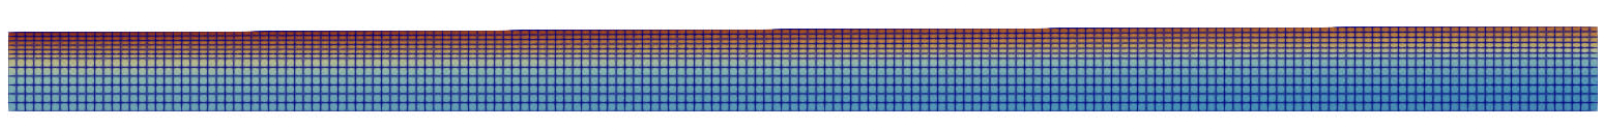
\includegraphics[width=0.9\textwidth]{../figs/ablation/end_time.png}
            \end{figure}}
        \end{column}
        \begin{column}{0.1\textwidth}
            \visible<3->{
            \begin{figure}
                \centering
                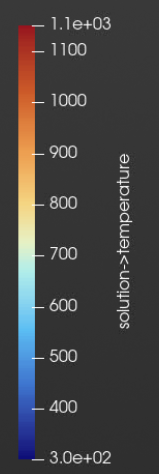
\includegraphics[width=0.9\textwidth]{../figs/ablation/temperature_axis.png}
            \end{figure}}
        \end{column}
    \end{columns}
\end{frame}

\begin{frame}{Hypersonic Thermal Protection Systems}
    \footnotesize
    \visible<1->{
    \textit{Reduced-physics model} (RPM) of ablating non-decomposing TPS via coarse-graining,}
    \begin{columns}
        \begin{column}{0.6\textwidth}
            \centering
            \begin{align*}
                \visible<2->{
                \text{Lumped-Capacitance Model: }& \vA(\vw)\dot{\bvu} = \vB(\vw)\bvu + \bar{\vf}(t)\\}
                \visible<3->{
                \text{1-D Surface Recession Model: }& \dot{\vw} = \vXi\bvu - \hat{\vf}\\}
                \visible<4->{
                \text{Reduced-Physics Model: }& \bar{\vA}(\bvx)\dot{\bvx} = \bar{\vB}(\bvx)\bvx + \bar{\vF}(t)}
            \end{align*}
            \visible<5->{
            \begin{gather*}
                \bar{\vA}(\bvx) = \begin{bmatrix}
                    \vA(\vw) & \boldsymbol{0}\\
                    \boldsymbol{0} & \vI
                \end{bmatrix}, \bar{\vB}(\bvx) = \begin{bmatrix}
                    \vB(\vw) & \boldsymbol{0}\\
                    \vXi & \boldsymbol{0}
                \end{bmatrix}, \\
                \bar{\vF}(t) = \left[\bar{\vf}(t),-\hat{\vf}(t)\right]^\top, \bvx = \left[\bvu,\vw\right]^T
            \end{gather*}}
        \end{column}
        \begin{column}{0.4\textwidth}
            \vspace{-0.1in}
            \visible<6->{
            \begin{figure}
                \centering
                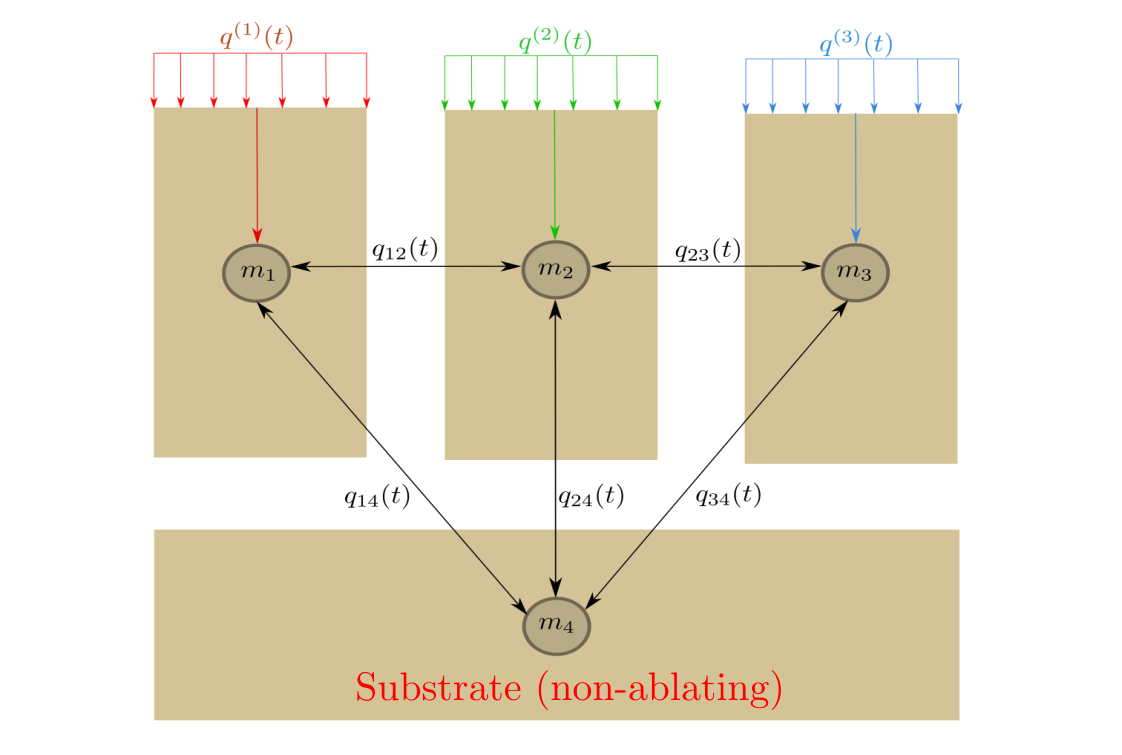
\includegraphics[width=1.0\textwidth]{../figs/ablation/lumped_mass_representation.png}
            \end{figure}}
        \end{column}
    \end{columns}
    \begin{center}
        \tiny
        $\vA$: capacitance matrix, $\vB$: conduction matrix, $\bvu$: average temperatures, $\vw$: one-dimensional component surface recession, $\vXi$: recession-rate matrix, $\hat{\vf}$: recession forcing, $\bar{\vf}$: heat flux forcing.
    \end{center}
\end{frame}

\begin{frame}{Hypersonic Thermal Protection Systems}
    \footnotesize
    \visible<1->{
    Relation between RPM and FOM exists via \textit{coarse-graining},}
    \visible<2->{
    \begin{figure}
        \centering
        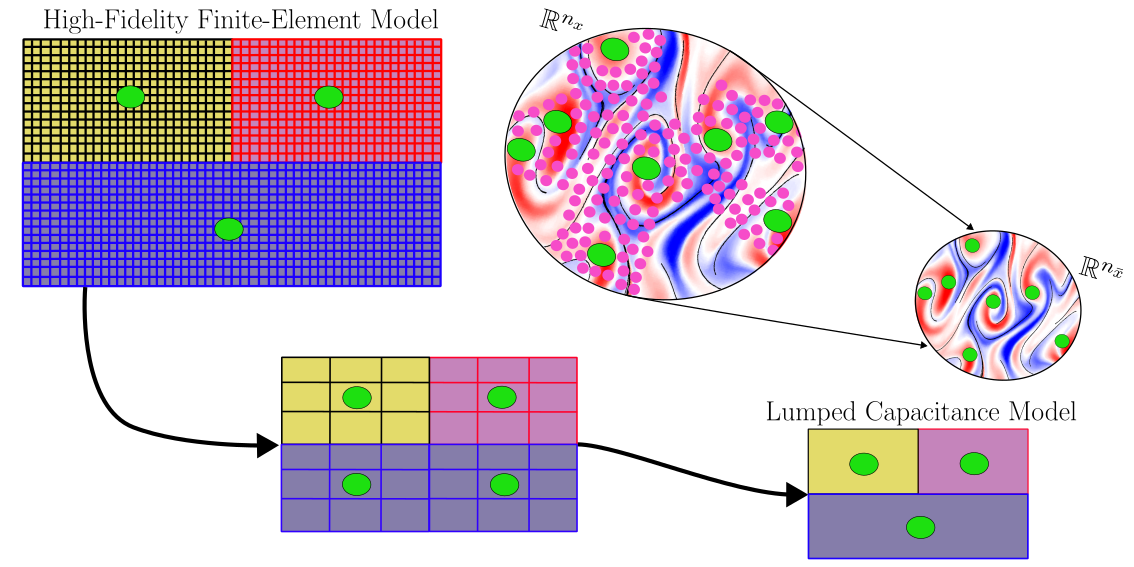
\includegraphics[width=0.8\textwidth]{../figs/ablation/coarse_graining_lcm.png}
    \end{figure}}
\end{frame}

\begin{frame}{Hypersonic Thermal Protection Systems}
    \footnotesize
    \visible<1->{
    Physics-infusion via \textit{Mori-Zwanzig},
    \vspace{-0.1in}}
    \begin{columns}
        \begin{column}{0.4\textwidth}
            \centering
            \visible<2->{
            \begin{graybox}{Markovian Dynamics}
                Lumped Capacitance Model
                \begin{equation*}
                    \vr^{(1)}\left(\bvx,t;\vp\right) = \vA(\vw)^{-1}\left[\vB(\vw)\bvu + \bar{\vf}(t)\right]
                \end{equation*}
            \end{graybox}}
        \end{column}
        \begin{column}{0.6\textwidth}
           \centering
           \visible<3->{
            \begin{graybox}{Memory Closure}
                \visible<4->{
                \begin{equation*}
                    \vkappa(t,s,\bvu) = \sum_{j=1}^{m}\mathcal{K}_j(t,s,\bvu)\left[\mathbf{p}_j + \vd_j(\bvu)\right]\phi_j(s,\bvu)
                \end{equation*}}
                \visible<5->{
                where,
                \begin{align*}
                    \mathcal{K}_j(t,s,\bvu) &= e^{-\int_{s}^{t}\left(\lambda_j + e_j(\bvu)\right)d\tau}\\
                    \phi_j(s,\bvu) &= \mathbf{q}_j^\top\bvu(s) + \mathbf{g}_j^\top(\bvu)\bvu(s) + \mathbf{r}_j^\top \bar{\mathbf{f}}(s)
                \end{align*}
                \vspace{-0.1in}}
            \end{graybox}}
        \end{column}
    \end{columns}
    \visible<6->{
    \vspace{-0.1in}
    \begin{graybox}{Markovian Reformulation}
        \visible<7->{
        Memory variables.
        \begin{equation*}
            \beta_j(t) = \int_{0}^{t}\mathcal{K}_j(s,\bvu)\phi_j(s,\bvu)ds
        \end{equation*}}
        \visible<8->{
        with dynamics,
        \begin{equation*}
            \dot{\beta}_j = -\left(\lambda_j + e_j(\bvu)\right)\beta_j(t) + \phi_j(t,\bvu)
        \end{equation*}
        \vspace{-0.1in}}
    \end{graybox}}
\end{frame}

\begin{frame}{Hypersonic Thermal Protection Systems}
    \footnotesize
    The physics-infused reduced-order model (PIROM) is written as,
    \vspace{-0.1in}
    \begin{graybox}{PIROM}
        \begin{align*}
            \vA(\vw)\dot{\bvu} &= \vB(\vw)\bvu + \left[\textcolor{red}{\vP} + \textcolor{red}{\vD}(\bvu)\right]\vbeta + \bar{\vf}(t)\\
            \dot{\vbeta} &= \left[\textcolor{red}{\vQ} + \textcolor{red}{\vG}(\bvu)\right]\bvu + \left[\textcolor{red}{\vE}(\bvu) - \textcolor{red}{\vLambda}\right]\vbeta + \textcolor{red}{\vR}\bar{\vf}(t)\rightarrow\text{follows the DG-FEM structure}
        \end{align*}
    \end{graybox}
    \begin{graybox}{Learnable Parameters}
        \begin{align*}
            \vLambda &= \text{diag}\left[\lambda_1,\lambda_2,\dots,\lambda_m\right]\in\mathbb{R}^{m\times m},\quad & \vP &= \left[\vp_1,\vp_2,\dots,\vp_m\right]\in\mathbb{R}^{N\times m}\\
            \vD(\bvu) &= \left[\vd_1(\bvu),\vd_2(\bvu),\dots,\vd_m(\bvu)\right]\in\mathbb{R}^{N\times m},\quad & \vQ &= \left[\vq_1,\vq_2,\dots,\vq_m\right]\in\mathbb{R}^{m\times N}\\
            \vG(\bvu) &= \left[\vg_1(\bvu),\vg_2(\bvu),\dots,\vg_m(\bvu)\right]\in\mathbb{R}^{m\times N},\quad & \vR &= \left[\vr_1,\vr_2,\dots,\vr_m\right]\in\mathbb{R}^{m\times N}\\
            \vE(\bvu) &= \text{diag}\left[e_1(\bvu),e_2(\bvu),\dots,e_m(\bvu)\right]\in\mathbb{R}^{m\times m}
        \end{align*}
    \end{graybox}
\end{frame}